\chapter{Methodology}
In this chapter we will explore the approaches followed to plan, organise, manage and develop the project. We will discuss the methodologies that were adapted and combined to complete the research and development of the project along with why they were implemented. This section aims to give insight to the reader how the project transformed from research to final software while collaborating as a team.

Throughout our four years at GMIT a major emphasis was always placed on the importance of software development methodologies and the importance of choosing the most suitable methodology for a given project;. There are numerous  methodologies that have all been extensivly explore such as Waterfall, RAD (Rapid Application Development) and Extreme Programming to name a few. For this project we chose the main modern leader also based on the methodologies used by our employers, a concept known as Agile programming.


% ========================== Development approach  ========================== 
\section{Agile development approach}
Agile Software Development is a concept that allows a product be delivered to the customer in incremental releases while also being highly flexiable, allowing requiremnts to change and the scope of the project to increase without major consequences on the design or current task.

We chose Agile as it stood out and had many benefits to our own project:

\begin{figure}[H]
\begin{minipage}{.5\textwidth}  %listing bloc will have 50% of the line width 
\lstset{linewidth = 4cm, breaklines=true} %set your listing lines widths, and set breaklines to true
\begin{itemize}
\item Develop small, incremental releases
\item Active user involvement
\item Evolving requirements
\item High level requirements
\end{itemize}

\end{minipage}
\qquad %space between listing bloc and the figure
\begin{minipage}{0.4\textwidth} %figure will have the remaning 40% of the line width
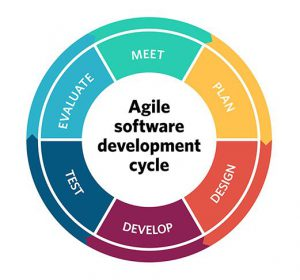
\includegraphics[scale=.4]{img/agile.jpg} %the image must be resized or scaled if needed
\caption{caption}
\end{minipage}
\end{figure}

Firstly as we were exploring all new languages, frameworks and libraries Agile allowed us to easily continuously integrate new features as our knowledge portfolio grew. Another major advantage was that this approach allowed us to have a working model every week rather than releasing the project in one release as would be in the Waterfall methodology. This alone gave us the opportunity to review each weeks progress while also receive continuous feedback from our mentors.

From the outset of the planning phase the main requirements and features of the software were identified. Subsequently we broke these features down into sub tasks which enabled complex tasks to be completed with simplicity.   


% ========================== KanBan  ========================== 
\subsection{KanBan}
The Kanban Method is a means to design, manage, and improve flow systems for knowledge work. The method also allows organizations to start with their existing workflow and drive evolutionary change. They can do this by visualizing their flow of work, limit work in progress (WIP) and stop starting and start finishing.

The Kanban Method gets its name from the use of kanban - visual signaling mechanisms to control work in progress for intangible work products.

% ========================== Version Control  ========================== 
\section{Version Control}
Use of github, branches , KanBan project section to track progress

% ========================== Choice of tech  ========================== 
\section{Choice of tech }
tech used and why
 Selection criteria for algorithms, languages, platforms and technolo-gies.
 
% ========================== Testing , pass fail metrics  ========================== 
\section{Testing , pass fail metrics}
how we planned to test, what did we deternmine wwas a pass or fail

Check out the nice graphs in Figure \ref{tikz:graphs}, and the nice diagram in Figure \ref{tikz:mydiagram}.

\begin{figure}
  \centering
  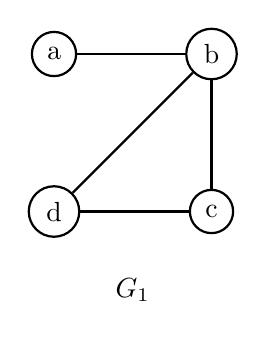
\begin{tikzpicture}
  \begin{scope}[every node/.style={circle,thick,draw}]
  \node (a) at (0,2) {a};
  \node (b) at (2,2) {b};
  \node (c) at (2,0) {c};
  \node (d) at (0,0) {d};
  \end{scope}
  \begin{scope}[every edge/.style={draw=black,thick}]
  \path (a) edge (b);
  \path (b) edge (c);
  \path (b) edge (d);
  \path (c) edge (d);
  \end{scope}
  \node () at (1,-1) {$G_1$};
  \end{tikzpicture}
  \hspace{1.5cm}
  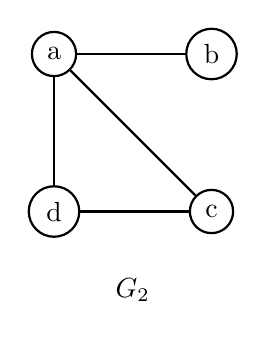
\begin{tikzpicture}
  \begin{scope}[every node/.style={circle,thick,draw}]
  \node (1) at (0,2) {a};
  \node (2) at (2,2) {b};
  \node (3) at (2,0) {c};
  \node (4) at (0,0) {d};
  \end{scope}
  \begin{scope}[every edge/.style={draw=black,thick}]
  \path (1) edge (2);
  \path (1) edge (3);
  \path (1) edge (4);
  \path (3) edge (4);
  \end{scope}
  \node () at (1,-1) {$G_2$};
  \end{tikzpicture}
  \caption{Nice pictures}
  \label{tikz:graphs}
\end{figure}


\begin{figure}
  \centering
  \begin{tikzpicture}[node distance=6cm]
  \node (a) [rect] {A Big Blue Block};
  \node (b) [oval, right of=a] {And His Oval Friend};
  \draw [line] (a) -- (b);
  \end{tikzpicture}
  \caption{Nice pictures}
  \label{tikz:graphs}
\end{figure}